\documentclass{article}

% New commands declaration

\usepackage[frenchb]{babel}
\usepackage[T1]{fontenc}

\usepackage{natbib,bibentry}
\usepackage{color}
\usepackage{yfonts}
\usepackage{graphicx}
\usepackage{epsfig,subfigure}
\usepackage{amsmath,amssymb,amsfonts}
\usepackage{calc}

\usepackage{float}
\usepackage{array}
\newcolumntype{L}[1]{>{\raggedright\let\newline\\\arraybackslash\hspace{0pt}}m{#1}}
\newcolumntype{C}[1]{>{\centering\let\newline\\\arraybackslash\hspace{0pt}}m{#1}}
\newcolumntype{R}[1]{>{\raggedleft\let\newline\\\arraybackslash\hspace{0pt}}m{#1}}


\DeclareGraphicsExtensions{.eps, .jpg, .png}

\parindent = 0mm

\bibliographystyle{plain}

\hoffset = -20mm
\voffset = -25mm
\textwidth = 160mm
\textheight = 240mm

\newcommand{\expect}{{\rm I \mkern-2.5mu \nonscript\mkern-.5mu E}}
\newcommand{\equaldef}{\stackrel{d}{=}}
\newcommand{\argmax}{\operatornamewithlimits{argmax}}

\newcommand{\dnu}{16}
\newcommand{\solskip}{10mm}

\newcommand{\debutrep}[1]{\color{blue}\begin{center} \hrulefill \textbf{ #1 } \hrulefill \end{center} }
\newcommand{\finrep}{\vspace*{5mm}\hfill $\square$\color{black}\vspace*{5mm}}


\begin{document}

\baselineskip = 4mm
\title{Traitement des Signaux Aléatoires \\
Estimation de densités de probabilité}
\author{\textbf{4 ETI -- CPE Lyon }\\[3mm]
{Travaux Pratiques TSA}}
\date{}

\maketitle

\noindent\fbox{
\parbox{\linewidth-2\fboxrule-2\fboxsep}
{ 
\vspace*{2mm}
{\large\bf Noms, Prénoms: LANGUILLE Antoine, BURNOT Jean-Christophe }\\[3mm]
{\large\bf Groupe: D}\\[3mm]
{\large\bf Date: 21 Novembre 2022}\\[2mm]}}
\vspace*{5mm}


\textbf{\Large Objectifs du TP}\\[4mm]

\begin{list}{-}{\setlength{\leftmargin}{3mm} \setlength{\labelwidth}{20mm} \setlength{\labelsep}{2mm} \setlength{\itemsep}{1mm} }
\item Synthèse et filtrage de processus aléatoires
\item Estimation empirique de densités de probabilités de différents processus aléatoires
\item Filtrage passe-bas de processus non gaussiens.
\end{list}

\vspace*{5mm}
\noindent\fbox{\parbox{\linewidth-2\fboxrule-2\fboxsep}{ \textbf{Consignes:}\\[-2mm]
\begin{list}{-}{\setlength{\leftmargin}{3mm} \setlength{\labelwidth}{20mm} \setlength{\labelsep}{2mm} \setlength{\itemsep}{1mm} }
\item Le répertoire de travail sera exclusivement sur le compte d'un des membres du binôme (changer le répertoire courant de Matlab®). Mais pour certains traitements, on fera appel à des fonctions pré- programmées. Les fonctions utiles sont accessibles sur CPe-campus dans le cours {\tt Traitement des signaux aléatoires}, rubrique {\tt Travaux Pratiques}. Récupérer les fichiers {\tt .m}.
\item Utiliser la trame de {\tt compte-rendu} fournie en répondant directement aux questions dans  les espaces ménagés à cet effet. 
\item Regrouper dans un fichier annexe (type {\tt word} ou {\tt text}) les Codes  Matlab® développés ainsi que les Figures obtenues. 
\textbf{Veiller à associer systématiquement une légende explicite à chaque Figure ou Tableau}. 
\item \textbf{Préparation obligatoire} (une seule par binôme) à rédiger directement sur le {\tt compte-rendu} et à fournir en début de séance
\end{list}
 }}

\vspace*{5mm}
\section{Préparation}

\textbf{Il faudra avoir pris connaissance de la totalité de l'énoncé et de la documentation des diverses fonctions Matlab fournie en Annexe.}\\

Pour estimer la densité de probabilité d'un signal aléatoire $\mathbf{x}$, on s'appuie ici sur l'histogramme d'une seule réalisation échantillonnée du signal aléatoire. Soient $\left(x[n] = x(n\cdot T_s) \right)_{n=1,\ldots,N}$, la série temporelle correspondante échantillonnée à la fréquence $F_s = T_S^{-1}$:
$$
\widehat{p_{\mathbf{x}}}(x) = \frac{\mbox{Nbre d'échantillons compris dans l'intervalle } \left[ x-\frac{\Delta x}{2},x+\frac{\Delta x}{2}\right]}{N\,\Delta x}.
$$

\begin{list}{}{\setlength{\leftmargin}{2mm} \setlength{\labelwidth}{0mm} \setlength{\labelsep}{3mm} \setlength{\itemsep}{1mm} }
\item[\textbf{Question 1}] Quelles propriétés le signal aléatoire $\mathbf{x}$ doit il vérifier:
\begin{list}{-}{\setlength{\leftmargin}{3mm} \setlength{\labelwidth}{20mm} \setlength{\labelsep}{2mm} \setlength{\itemsep}{1mm} }
\item   pour que les échantillons  $\left(x[n]\right)_{n=1,\ldots N}$ soient identiquement distribués (i.e. suivent tous la même loi, quelque soit l'instant $n$)?

\debutrep{réponse ci-dessous}
Pour que les échantillons soient identiquement distribués, il faut que le signal soit strictement stationnaire.
\finrep

\item   pour que les échantillons  $\left(x[n]\right)_{n=1,\ldots N}$ soient décorrélés?

\debutrep{réponse ci-dessous}
Il faut que $\mathbb{E}\{X(t_1)X(t_2)\} = 0$
\finrep


\item  pour que la décorrélation des échantillons $\left(x[n]\right)_{n=1,\ldots N}$ entraine  également leur indépendance?

\debutrep{réponse ci-dessous}
La décorrélation entraine l'indépandance dans le cas d'un signal gaussien.
\finrep
 
\end{list}

\item[\textbf{Question 2}] Sans calculs, indiquer quelle est l'influence du choix de $\Delta x$ sur le biais et sur la variance de l'estimation $\widehat{p_{\mathbf{x}}}(x)$.

\debutrep{réponse ci-dessous}
La largeur des classes $\Delta x$ illustre le compromis biais-variance
\begin{itemize}
    \item Si $\Delta x$ augmente, plus d'échantillons tombent dans la même classe, l'histogramme se rapproche plus d'un moyenneur. Le biais augmente donc, la densité de probabilité tendant vers l'espérance du signal. La variance se réduit alors.
    
    \vspace*{3mm}
    \begin{center}
    
        $\Delta x$ augmmente $\Rightarrow$ biais augmente, variance diminue
    \end{center}
    \vspace*{3mm}

    \item Si $\Delta x$ diminue, les classes sont plus nombreuses et plus petites, leur valeur dépend alors davantage des échantillons individuels, la variance augmente donc. Au contraire, le biais se réduit, la forme de l'histogramme se rapprochant plus de celle de la densité de probabilité.
   
    \vspace*{3mm}
    \begin{center}
        $\Delta x$ diminue $\Rightarrow$ biais diminue, variance augmente
    \end{center}


\end{itemize}
\finrep
 
\item[\textbf{Question 3}] Quelles opérations (arithmétiques simples, il ne s'agit pas de filtrage ici!) permettent de synthétiser un processus gaussien de moyenne $m_2$ et d'écart-type $\sigma_2$ à partir d'un processus gaussien stationnaire de moyenne $m_1 \neq m_2$ et d'écart-type $\sigma_1 \neq \sigma_2$?

\debutrep{réponse ci-dessous}
 Les quatres opérations élémentaires suffisent $(+,-,\times,\div)$.
On procède en 2 étapes:
\begin{itemize}
    \item On centre réduit la gaussienne $G_1 \sim Gau(m_1, \sigma_1)$ en $G_0 \sim Gau(0, 1)$ par l'opération 
    \[G_0 = \frac{G_1 - m_1}{\sigma_1}\]
    \item On dilate puis décale la loi gaussienne centrée réduite que l'on vient de calculer pour obtenir une loi gaussienne $G_2 \sim Gau(m_2,\sigma_2)$ grâce à l'opération
    \[ G_2 = G_0 \times \sigma_2 + m_2\]
\end{itemize}
L'opération finale s'exprime donc
\[ G_2 = \frac{G_1 - m_1} {\sigma_1}\sigma_2 + m_2 \]
 \finrep
 

\item[\textbf{Question 4}] Le {\bf Kurtosis} est un indice qui permet de mesurer le caractère normal (gaussien) d'une série d'échantillons d'une variable aléatoire. Il est défini par le rapport: ${\displaystyle K=\frac{\mathbb{E}\left\{\mathbf{x}^4\right\}}{\mathbb{E}^2\left\{\mathbf{x}^2\right\}}}$

On rappelle que si $\mathbf{x}$ est gaussien et \underline{centré}, alors
\begin{eqnarray*}
\mathbb{E}\{x(t_1)x(t_2)x(t_3)x(t_4)\} & = & \mathbb{E}\{x(t_1)x(t_2)\} \, \mathbb{E}\{x(t_3)x(t_4)\} +  \mathbb{E}\{x(t_1)x(t_3)\}\,\mathbb{E}\{x(t_2)x(t_4)\}  \ldots \\
& &+ \,\mathbb{E}\{x(t_1)x(t_4)\}\,\mathbb{E}\{x(t_2)x(t_3)\} 
\end{eqnarray*}
Montrer alors que dans le cas d'un signal aléatoire gaussien, centré et stationnaire, le Kurtosis vaut 3.


\debutrep{réponse ci-dessous}

On a 
\[
    K = \frac{
        \mathbb{E} \{x^4\}
   }{
        \mathbb{E}^2\{x^2\}
    }
     = \frac{
        \mathbb{E}\{x^2\} + \mathbb{E}\{x^2\}\times\mathbb{E}\{x^2\} + \mathbb{E}\{x^2\}\times\mathbb{E}\{x^2\} + \mathbb{E}\{x^2\}\times\mathbb{E}\{x^2\}
   }{
        \mathbb{E}^2\{x^2\}
    }
    = \frac{
        3\mathbb{E}^2\{x^2\}
    }{
        \mathbb{E}^2\{x^2\}
    }
    = 3
\]

\finrep
 

\item[\textbf{Question 5}] Soit $\mathbf{x}(t)$  un bruit gaussien de valeur moyenne $m_B$ et d'écart-type $\sigma_B$. \\
Soit $\mathbf{y}(t)$ un signal carré d'amplitude $A$, centré, périodique de période $T_0$, de rapport cyclique égal à 1 et retardé par rapport à l'origine d'un retard $\tau$ uniformément distribué entre $0$ et $T_0$.\\
Donner l'expression de la densité de probabilité de la somme $\mathbf{z}(t) = \mathbf{x}(t)+\mathbf{y}(t)$.


\debutrep{réponse ci-dessous}
On a $x(t) \sim Gau(m_B, \sigma_B)$.
\vspace*{3mm}

et $y(t) = $
\begin{cases}
 & $\text{Amplitude: } A$ \\
 & $\text{Centré: } m=0$ \\
 & $\text{Période: } T_0$ \\
 & $\alpha=1 \text{(fonction constante)}$ \\
 & $\text{Retard: } \tau$ 
\end{cases}
$\Leftrightarrow y(t) = A$.

\vspace*{3mm}
La densité de probabilité de $z(t)=x(t) + y(t)$ n'est autre qu'une gaussienne de même écart-type $\sigma_B$ que $x(t)$ mais d'espérance $m_B+A$.

\finrep
 
\end{list}

\clearpage

\begin{center}
{\Large Traitement des Signaux Aléatoires} \\
{\Large Estimation de densités de probabilité}
\textbf{4 ETI -- CPE Lyon }\\[3mm]
{Travaux Pratiques TSA}\\[3mm]
{}
\end{center}

\noindent\fbox{
\parbox{\linewidth-2\fboxrule-2\fboxsep}
{ 
\vspace*{2mm}
{\large\bf Noms, Prénoms: LANGUILLE Antoine, BURNOT Jean-Christophe}\\[3mm]
{\large\bf Groupe: D}\\[3mm]
{\large\bf Date: 21 Novembre 2022}\\[2mm]}}
\vspace*{5mm}

\section{Bruit gaussien filtré, échantillonné}

On souhaite générer un bruit gaussien $x_3(t)$ blanc dans la bande $[-B,B]$, de moyenne $m_3$ non nulle et d'écart-type $\sigma_3 > 1$. Pour cela, on applique la procédure décrite dans la préparation (Question 3) et schématisée ci-dessous:\\

\begin{center}
\includegraphics[width=0.7\columnwidth]{TPTSA1-synthese.png}
\end{center}

où $x_1(t)$ est un bruit blanc gaussien, centré, d'écart-type $\sigma_1=1$.

\subsection{Programmation}

\textbf{Programmer deux fonctions Matlab distinctes dont vous reproduirez  les codes ci-dessous.}

\subsubsection{Fonction synthèse des signaux aléatoires}

\begin{list}{$\bullet$}{\setlength{\leftmargin}{3mm} \setlength{\labelwidth}{20mm} \setlength{\labelsep}{2mm} \setlength{\itemsep}{1mm} }
\item Paramètres d'entrée:
\begin{list}{-}{\setlength{\leftmargin}{3mm} \setlength{\labelwidth}{20mm} \setlength{\labelsep}{2mm} \setlength{\itemsep}{1mm} }
\item le nombre $N$ d'échantillons à générer
\item la largeur de bande $B$ du filtre passe-bas
\item la moyenne $m_3$ et l'écart-type $\sigma_3$ du bruit $x_3(t)$.
\end{list}
\item Traitements à effectuer dans la fonction:
\begin{list}{-}{\setlength{\leftmargin}{3mm} \setlength{\labelwidth}{20mm} \setlength{\labelsep}{2mm} \setlength{\itemsep}{1mm} }
\item génération d'une séquence $x_1(t)$ de bruit gaussien échantillonné (à la fréquence $F_s$), centré et d'écart-type $\sigma_1=1$
\item synthèse d'un filtre de {\em Butterworth} de type passe-bas, de fréquence de coupure $f_c$ correspondant à la largeur de bande $B$ et d'ordre $m=8$
\item filtrage du bruit $x_1(t)$ par le filtre passe-bas pour obtenir le bruit filtré $x_2(t)$
\item transformation de $x_2(t)$ pour obtenir $x_3(t)$ de  valeur moyenne $m_3$ et d'écart-type $\sigma_3$.
\end{list}
\item Variables de sortie:
\begin{list}{-}{\setlength{\leftmargin}{3mm} \setlength{\labelwidth}{20mm} \setlength{\labelsep}{2mm} \setlength{\itemsep}{1mm} }
\item les vecteurs des échantillons de $x_1$, $x_2$ et $x_3$
\item les coefficients de la fonction de transfert du filtre passe-bas (coefficients des polynômes $A(z)$ et $B(z)$).
\end{list}
\end{list}


\debutrep{code ci-dessous}
 \begin{verbatim}
function [X1, X2, X3, A, B] = synthesize(N, B, m, s)
    
    Fs = 1e3;   % Fréquence d'échantillonnage 1kHz

    X1 = randn(N,1);            % Bruit gaussien centré réduis
    fc = B/(Fs/2);              % Fréquence normalisée pour filtre
    [B, A] = butter(8, fc);     % Génération du filtre
    X2 = filter(B, A, X1);      % Filtrage

    % X2 n'est plus centré réduis après filtrage
    X2 = (X2-mean(X2))/std(X2); % On centre réduis X2
    
    % On inverse l'opération de centrage-réduction
    X3 = s*X2 + m;      % Dilatation décalage du bruit centré réduis
end
 \end{verbatim}
\finrep
 
\subsubsection{Fonction Calcul d'histogramme}

\begin{list}{$\bullet$}{\setlength{\leftmargin}{3mm} \setlength{\labelwidth}{20mm} \setlength{\labelsep}{2mm} \setlength{\itemsep}{1mm} }
\item Paramètres d'entrée:
\begin{list}{-}{\setlength{\leftmargin}{3mm} \setlength{\labelwidth}{20mm} \setlength{\labelsep}{2mm} \setlength{\itemsep}{1mm} }
\item le vecteur des $N$ échantillons d'un signal aléatoire $x(t)$
\item paramètre \textbf{optionnel}: $M$ le nombre d'intervalles imposés pour le calcul de l'histogramme
\end{list}
\item Traitements à effectuer:
\begin{list}{-}{\setlength{\leftmargin}{3mm} \setlength{\labelwidth}{20mm} \setlength{\labelsep}{2mm} \setlength{\itemsep}{1mm} }
\item si le nombre d'intervalles $M$ n'est pas spécifié:
\begin{list}{$\circ$}{\setlength{\leftmargin}{3mm} \setlength{\labelwidth}{20mm} \setlength{\labelsep}{2mm} \setlength{\itemsep}{1mm} }
\item appliquer la règle empirique de calcul {\em optimal} de $\Delta x$ (vue en TD)
\item calculer le centre de chaque intervalle de l'histogramme correspondant à ce choix de $\Delta x$
\item calculer l'histogramme correspondant
\end{list}
\item si le nombre d'intervalles $M$ est spécifié:
\begin{list}{$\circ$}{\setlength{\leftmargin}{3mm} \setlength{\labelwidth}{20mm} \setlength{\labelsep}{2mm} \setlength{\itemsep}{1mm} }
\item déterminer la largeur des intervalles $\Delta x$ correspondant à ce choix de $M$
\item calculer l'histogramme correspondant
\end{list}
\item déduire de l'histogramme calculé une estimation de la densité de probabilité de $\mathbf{x}$
\item afficher \underline{dans la figure et le graphe courants} la densité de probabilité estimée
\item labéliser les axes en indiquant la valeur de $\Delta x$ utilisée (et préciser si celle-ci est {\em optimale} ou {\em imposée}). Donner un titre pertinent (distinctif) au graphe.
\end{list}
\item Variables de sortie:
\begin{list}{-}{\setlength{\leftmargin}{3mm} \setlength{\labelwidth}{20mm} \setlength{\labelsep}{2mm} \setlength{\itemsep}{1mm} }
\item le vecteur des valeurs de la densité de probabilité estimée
\item le vecteur des centres d'intervalles calculés
\end{list}
\end{list}

\debutrep{code ci-dessous}
 \begin{verbatim}
 function [dp,cbins] = drawhist(X,M)
    if ~exist('M','var')
        % Valeur par défaut si M non fourni
                
        % Largeur ayant le meilleur compromis biais-variable
        dx = 3.49 * std(X) * length(X) ^ (-1/3);
        
        M = ceil((max(X) - min(X)) / dx); %nombre de bins associé à dx
        msg = "optimale";
    else
        % M fourni
        dx = (max(X) - min(X)) / M;     % On calcule dx à partir de M
        msg = "imposée";
    end
    
    [counts, cbins] = hist(X, M);    % On précise ici le nombre de bins de l'histogramme

    dp = counts./(length(X)*dx);    % On normalise l'histogramme en densité de probabilités
    
    % Affichage
    bar(cbins, dp); 
    hold on;
    xlabel(sprintf("\\Deltax = %f (%s)",dx, msg));
    title(sprintf("Estimation DP (\\Deltax=%d)", dx));
end

 \end{verbatim}
\finrep

\subsection{Expérimentation}

\subsubsection{Cas général}

On supposera que le signal est échantillonné à la fréquence $F_s = 1\,KHz$. Ce choix est il important? Pourquoi?

\debutrep{réponse ci-dessous}
 La fréquence d'échantillonnage est importante, car si elle est trop faible, il y aura repliement spectral (Théorème de Shannon-Nyquist).
 \finrep
 
Dans les conditions suivantes:
\begin{list}{-}{\setlength{\leftmargin}{3mm} \setlength{\labelwidth}{20mm} \setlength{\labelsep}{2mm} \setlength{\itemsep}{1mm} }
\item $N=1000$ échantillons de signal
\item Filtre passe-bas avec $B=100\,Hz$ (ordre $m=8$)
\item $m_3 \neq 0$ et $\sigma_3 >1$ (choix libres que l'on précisera clairement dans le compte-rendu)
\item choix empirique {\em optimal} de la largeur $\Delta x$ des intervalles,
\end{list}

\textbf{afficher ci-dessous, sur une même figure partagée en $2 \times 4$ sous-graphes} ({\em subplots}):
\begin{list}{-}{\setlength{\leftmargin}{3mm} \setlength{\labelwidth}{20mm} \setlength{\labelsep}{2mm} \setlength{\itemsep}{1mm} }
\item sur la première ligne: les séries temporelles $x_1(k.T_s)$, $x_2(k.T_s)$ et $x_3(k.T_s)$, ainsi que le module du gain complexe du filtre passe-bas
\item sur la deuxième ligne: sous chacune des 3 séries temporelles, les densités de probabilité estimées auxquelles on superposera les densités théorique correspondantes. \textbf{Donner aussi le code utilisé pour calculer et afficher ces d.d.p. théoriques.}
\end{list}

\newpage
\debutrep{figure ci-dessous} 
\begin{figure}  [H]
    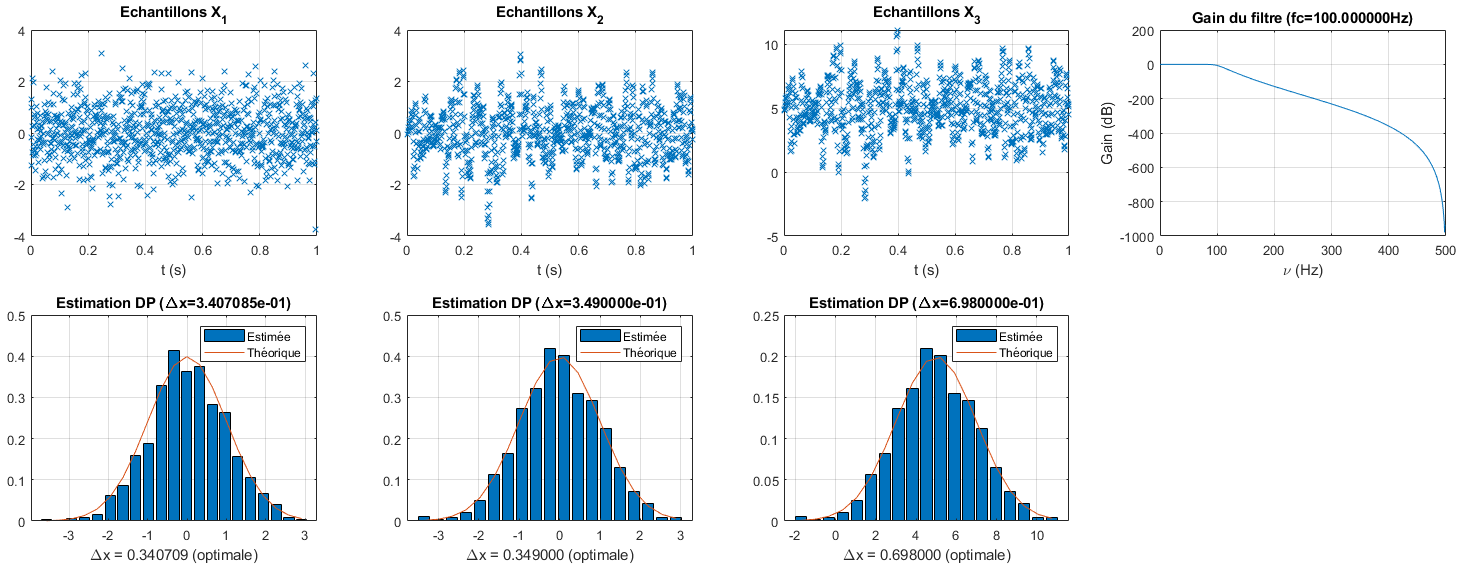
\includegraphics[width=1.15\columnwidth]{plot-basique.png}
    \caption{Signaux et histogrammes associés}
\end{figure}
\finrep
 
\debutrep{code ci-dessous}
\begin{verbatim}
%% TP 1: Estimation de densités de probabilité

clear variables;
close all;

Fs = 1e3;   % 1kHz

N = 1e3;    % 1000 échantillons
B = 100;    % 100Hz

fc = B;     % Fréquence de coupure du filtre

% Espéarance et écart-type du bruit X3
m = 5;      
s = 2;

% On charche dx optimal (on ne précise donc pas M)
[X1, X2, X3, A, B] = synthesize(N, B, m, s);

% Affichage
figure(1);
subplot(2,4,1);
x = 0 : 1/Fs : (length(X1)-1)/Fs;
plot(x, X1, 'x');
title("Echantillons X_1");
xlabel("t (s)");

subplot(2,4,2);
x = 0 : 1/Fs : (length(X2)-1)/Fs;
plot(x, X2, 'x');
title("Echantillons X_2");
xlabel("t (s)");


subplot(2,4,3);
x = 0 : 1/Fs : (length(X3)-1)/Fs;
plot(x, X3, 'x');
title("Echantillons X_3");
xlabel("t (s)");


subplot(2,4,4);
[h,f] = freqz(B, A, N, Fs);
plot(f, 20*log(abs(h)));
title(sprintf("Gain du filtre (fc=%fHz)", fc));
xlabel("\nu (Hz)");
ylabel("Gain (dB)");

% Gaussienne
gauss = @(x, mu, sig) (1/(sig*sqrt(2*pi)) * exp( -(x-mu).^2/(2*sig^2) ));

subplot(2,4,5);
[dp1, cbins1] = drawhist(X1);
plot(cbins1, gauss(cbins1, 0, 1));
legend('Estimée','Théorique');

subplot(2,4,6);
[dp2, cbins2] = drawhist(X2);
plot(cbins2, gauss(cbins2, 0, 1));
legend('Estimée','Théorique');

subplot(2,4,7);
[dp3, cbins3] = drawhist(X3);
plot(cbins3, gauss(cbins3, m, 2));
legend('Estimée','Théorique');

\end{verbatim}
\finrep

\newpage
 
Pour chacun des 3 processus, vérifier par la mesure sur les densités estimées et en utilisant des estimateurs empiriques (disponibles sous Matlab):
\begin{list}{}{\setlength{\leftmargin}{6mm} \setlength{\labelwidth}{20mm} \setlength{\labelsep}{2mm} \setlength{\itemsep}{1mm} }
\item[a)] la conformité entre moyennes mesurées et théoriques. Compléter la \textbf{Table \ref{tab:moyenne}} avec les valeurs mesurées.

\vspace*{4mm}

\begin{table}[H] % ======================================================================================
\setlength{\tabcolsep}{4mm}
\renewcommand{\arraystretch}{2}
\begin{tabular}{|p{30mm}|p{30mm}|p{30mm}|p{30mm}|}
\hline
& $\widehat{m_1}$ & $\widehat{m_2}$ & $\widehat{m_3}$ \\ \hline
Décrire une 1ère méthode de mesure  de la moyenne & 
\multicolumn{3}{p{90mm}|}
{
\debutrep{réponse et mesures ci-dessous}
On prend la valeur centrale de la classe ayant la plus grande probatilité.
\finrep
} \\ \hline
Mesure de la moyenne par la méthode 1 
& $\widehat{m_1} \approx -0.334$ 
& $\widehat{m_2} \approx -0.2403$ 
& $\widehat{m_3} \approx 4.519$ 
\\ \hline
Décrire une 2ème méthode de mesure  de la moyenne & 
\multicolumn{3}{p{90mm}|}
{
\debutrep{réponse et mesures ci-dessous}
On prend la valeur médianne des valeurs de nos échantillons.
\finrep
} \\ \hline
Mesure de la moyenne par la méthode 2 
& $\widehat{m_1} \approx -0.334$ 
& $\widehat{m_2} \approx -0.2403$ 
& $\widehat{m_3} \approx 4.519$ 
\\ \hline
\end{tabular}
\caption{Estimations de la valeur moyenne des signaux}
\label{tab:moyenne}
\end{table} % ======================================================================================

\newpage

\item[b)] idem pour les écart-type (avec \underline{au moins deux méthodes} de mesure distinctes que l'on détaillera). Compléter la \textbf{Table \ref{tab:ecart-type}} avec les valeurs mesurées.


\vspace*{4mm}

\begin{table}[H] % ======================================================================================
\setlength{\tabcolsep}{4mm}
\renewcommand{\arraystretch}{2}
\begin{tabular}{|p{30mm}|p{30mm}|p{30mm}|p{30mm}|}
\hline
& $\widehat{\sigma_1}$ & $\widehat{\sigma_2}$ & $\widehat{\sigma_3}$ \\ \hline
Décrire une 1ère méthode de mesure  de l'écart-type & 
\multicolumn{3}{p{90mm}|}
{
\debutrep{réponse et mesures ci-dessous}
On regarde les deux valeurs pour lesquelles la densité de probabilité atteint la moitié de la hauteur maximale de la courbe. L'écart entre ces deux valeurs constitue la "Largeur à mi hauteur" et est égale à environ $2.355\sigma$.
\finrep
} \\ \hline
Mesure de l'ecart-type par la méthode 1 
& $\widehat{\sigma_1} \approx 1.023628$ 
& $\widehat{\sigma_2} \approx 1.144940$ 
& $\widehat{\sigma_3} \approx 2.073252$ 
\\ \hline
Décrire une 2ème méthode de mesure  de l'écart-type & 
\multicolumn{3}{p{100mm}|}
{
\debutrep{réponse et mesures ci-dessous}
On regarde la valeur pour laquelles, l'aire sous la courbe centrée entre cette valeur et son opposée atteint $68.27\%$ de l'aire totale. Cette valeur est alors l'écart-type $\sigma$.
\finrep
} \\ \hline
Mesure de l'écart-type par la méthode 2 
& $\widehat{\sigma_1} \approx 1.240000$ 
& $\widehat{\sigma_2} \approx 1.236000$ 
& $\widehat{\sigma_3} \approx 2.398000$ 
\\ \hline
Décrire une 3ème méthode de mesure  de l'écart-type & 
\multicolumn{3}{p{100mm}|}
{
\debutrep{réponse et mesures ci-dessous}

\finrep
} \\ \hline
Mesure de l'écart-type par la méthode 3 
& $\widehat{\sigma_1} \approx $ 
& $\widehat{\sigma_2} \approx $ 
& $\widehat{\sigma_3} \approx $ 
\\ \hline
Décrire une 4ème méthode de mesure  de l'écart-type & 
\multicolumn{3}{p{100mm}|}
{
\debutrep{réponse et mesures ci-dessous}

\finrep
} \\ \hline
Mesure de l'écart-type par la méthode 4 
& $\widehat{\sigma_1} \approx $ 
& $\widehat{\sigma_2} \approx $ 
& $\widehat{\sigma_3} \approx $ 
\\ \hline
\end{tabular}
\caption{Estimations de l'écart-type}
\label{tab:ecart-type}
\end{table}
\end{list}

\newpage
\vspace*{4mm}
Lesquelles de ces méthodes vous paraissent les plus précises? Pourquoi?

\debutrep{réponse ci-dessous}
Pour l'espérance, la méthode de la médianne semble plus précise car au contraire de la méthode de la barre la plus haute. En effet la médianne tiens compte de la totalié des échantillons, là où la méthode de la barre la plus haute ne dépends que des échantillons tombant dans la classe considérée.

Pour l'écart-type, la méthode faisait appel à la l'aire sous la courbe semble la plus précise car elle requiert une intégrale de la densité de probabilité estimée et fait donc intervenir tous les échantillons dans toutes les classes. En revanche la méthode de la largeur à mi hauteur ne fait intervenir au plus que 3 échantillons (valeur maximale atteinte et les deux échantillons pour mesurer la largeur).
\finrep

\subsubsection{Influence de $N$}

On ne considère ici que le signal aléatoire $x_1(t)$, le nombre d'intervalles pour le calcul des histogrammes restant constant et égal à $M=20$. 

\begin{list}{}{\setlength{\leftmargin}{6mm} \setlength{\labelwidth}{20mm} \setlength{\labelsep}{2mm} \setlength{\itemsep}{1mm} }

\item[a)] Sur une même figure, afficher dans différents sous-graphes (pour une meilleure lisibilité des courbes, on pourra utiliser la commande {\tt stem.m} en lieu et place de la commande {\tt bar.m}), les densités de probabilité de $x_1(t)$ estimées pour plusieurs valeurs du nombre d'échantillons: pour cela faire varier dans une boucle {\tt for\ldots end}, le nombre $N$ de $2^4$ à $2^{11}$. Superposer systématiquement  les densités théoriques ainsi que les intervalles de précision théoriques $\mathbb{E}\{\widehat{p_{\mathbf{x}}}(x)\} \pm {\rm std}(\widehat{p_{\mathbf{x}}}(x))$ calculés en TD. Veiller à  commenter précisément chaque figure (légendes, labels,\ldots)\\
\textbf{Donner aussi le code Matlab de calcul de ces intervalles de confiance.} 


\debutrep{figures ci-dessous}
\begin{figure} [H]
    \centering
    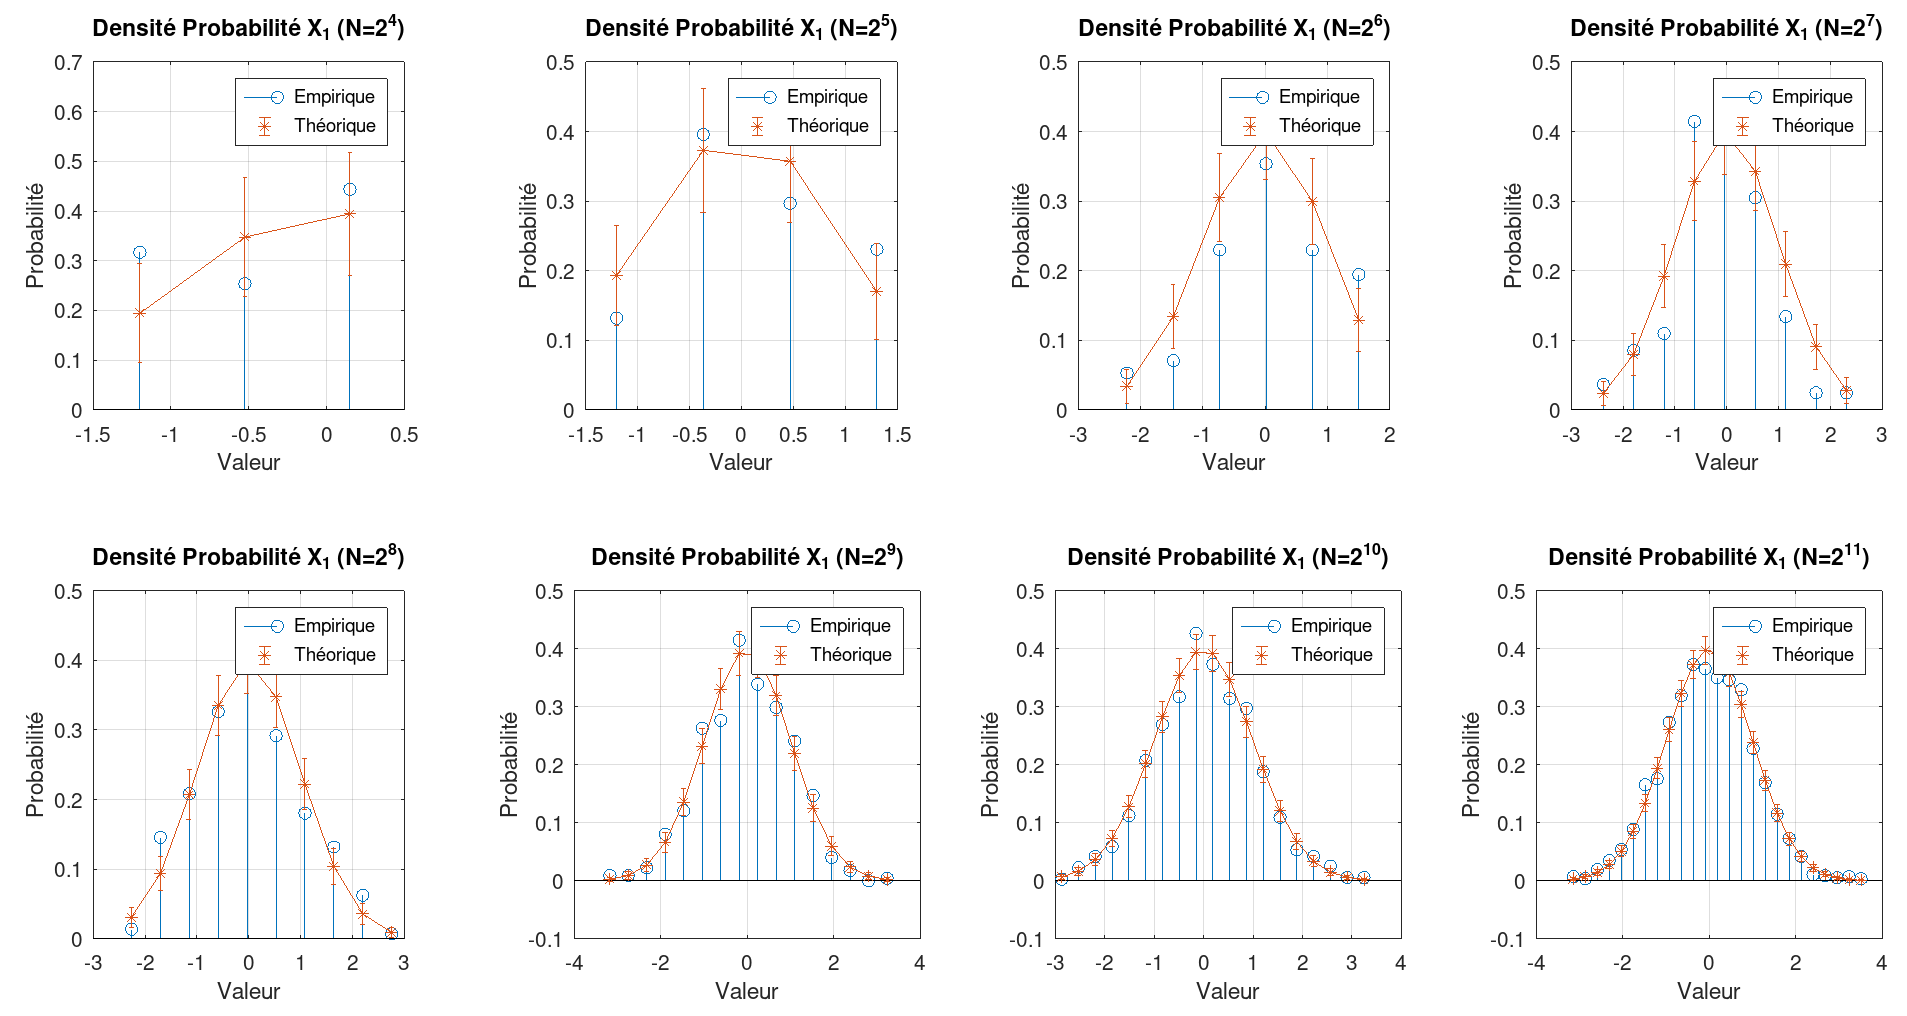
\includegraphics[width=1.15\columnwidth]{Nvar.png}
    \caption{Variation du nombre d'échantillons N}
\end{figure}

\finrep

\newpage
\debutrep{code ci-dessous}
\begin{verbatim}
% Variation du paramètre M

figure(2);

for i=4:11
  
  subplot(2,4,i-3);
  
  N = 2^i;
  [X1, X2, X3, Ac, Bc] = synthesize(N, B, m, s);
  
  
  % Affichage de la densité empirique
  [dp1, cbins1] = drawhist(X1);
  
  % Affichagege de ala densité théorique
  dp1_th = gauss(cbins1, 0, 1);
  
  % Calcul de l'espérance et de l'écart-type de chaque classe
  dx = 3.49 * std(X1) * length(X1) ^ (-1/3);
  
  Ex = dp1_th;                     % Formules de TD
  Vx = dp1_th/N .* (1/dx - dp1_th);
  
  Incert1 = sqrt(Vx);
  
  errorbar(cbins1, dp1_th, Incert1, '-*');
  
  title(sprintf("Densité Probabilité X_1 (N=2^{%d})", i));
  xlabel("Valeur");
  ylabel("Probabilité");
  legend("Empirique","Théorique");
  grid on;
  

end
\end{verbatim}
\finrep

\item[b)] Qualitativement, expliquez à partir de ces tracés, l'évolution de la variance (ou de l'écart-type) d'estimation.

\debutrep{réponse ci-dessous}
On observe que plus le nombre d'échantillons augmente, plus la densité de probabilité empirique se rapproche de la densité théorique. Les barres d'erreur se réduisent signifiant que l'espérance ne change pas (comme attendu) mais que l'écart-type et donc la variance diminue.
\finrep

\item [c)] Peut on conclure sur le biais d'estimation à partir de cette seule expérience? Expliquez.

\debutrep{réponse ci-dessous}
À partir de cette expérience seule, on ne peut conclure définitivement sur le biais ou la variance de cet estimateur. En effet l'estimateur ne dépend pas directement du paramètre N. Le seul paramètre inhérent à l'estimateur est le paramètre M. Les paramètres N, B, Fc... dépendent des signaux synthétisés.
\finrep

\item[d)] Quelle expérience faudrait il mener pour caractériser empiriquement et précisément le biais et la variance d'estimation?

\debutrep{réponse ci-dessous}
Pour caractériser le biais et la variance de l'estimateur, il faudrait cette fois-ci faire varier le paramètre M (et donc $\Delta x$). Pour chaque valeur de M, on effectue plusieurs estimation du même signal aléatoire pour estimer le biais et la variance.
\finrep


\end{list}

\subsubsection{Influence de $\Delta x$}

Ici encore, on ne s'intéresse qu'à $x_1(t)$ et à une de ses réalisations sur $N=1000$ points.

\begin{list}{}{\setlength{\leftmargin}{6mm} \setlength{\labelwidth}{20mm} \setlength{\labelsep}{2mm} \setlength{\itemsep}{1mm} }

\item[a)]  En faisant varier $M$, le nombre d'intervalles de l'histogramme, sur une plage incluant les 2 situations extrêmes (\textbf{que l'on indiquera et justifiera}), calculer et afficher (sur une même figure partagée en sous-graphes) les densités de probabilité estimées. Superposer les densités théoriques ainsi que les intervalles de précision.


\debutrep{réponse ci-dessous}
Les deux situations extrêmes sont:

\begin{itemize}
    \item $M=1$, une seule classe récupère tous les échantillons, l'estimateur se résume alors à un moyenneur. On s'attend donc à avoir une erreur d'estimation maximale (densité de probabilité constante très éloignée d'une gaussienne) mais une variance très faible.
    \vspace*{3mm}
    \item $M=N$, autant de classe que d'échantillons. L'estimation se rapproche au plus près de la densité théorique. Le biais est donc minimum mais chaque classe ne contenant que peu d'échantillons, la valeur de l'estimation varie beaucoup entre chaque estimation, la variance sera alors importante.
\end{itemize}
\vspace*{5mm}
Ansi, faire un balayage de $M=1$ à $M=N$ permet de bien voir l'évolution du biais et de la variance de l'estimateur.
\finrep

\newpage
\item[b)] Dans un dernier sous-graphe de la même figure, représenter la densité de probabilité estimée avec un choix optimal de $\Delta x$.

\debutrep{figures ci-dessous}
\begin{figure} [H]
    \centering
    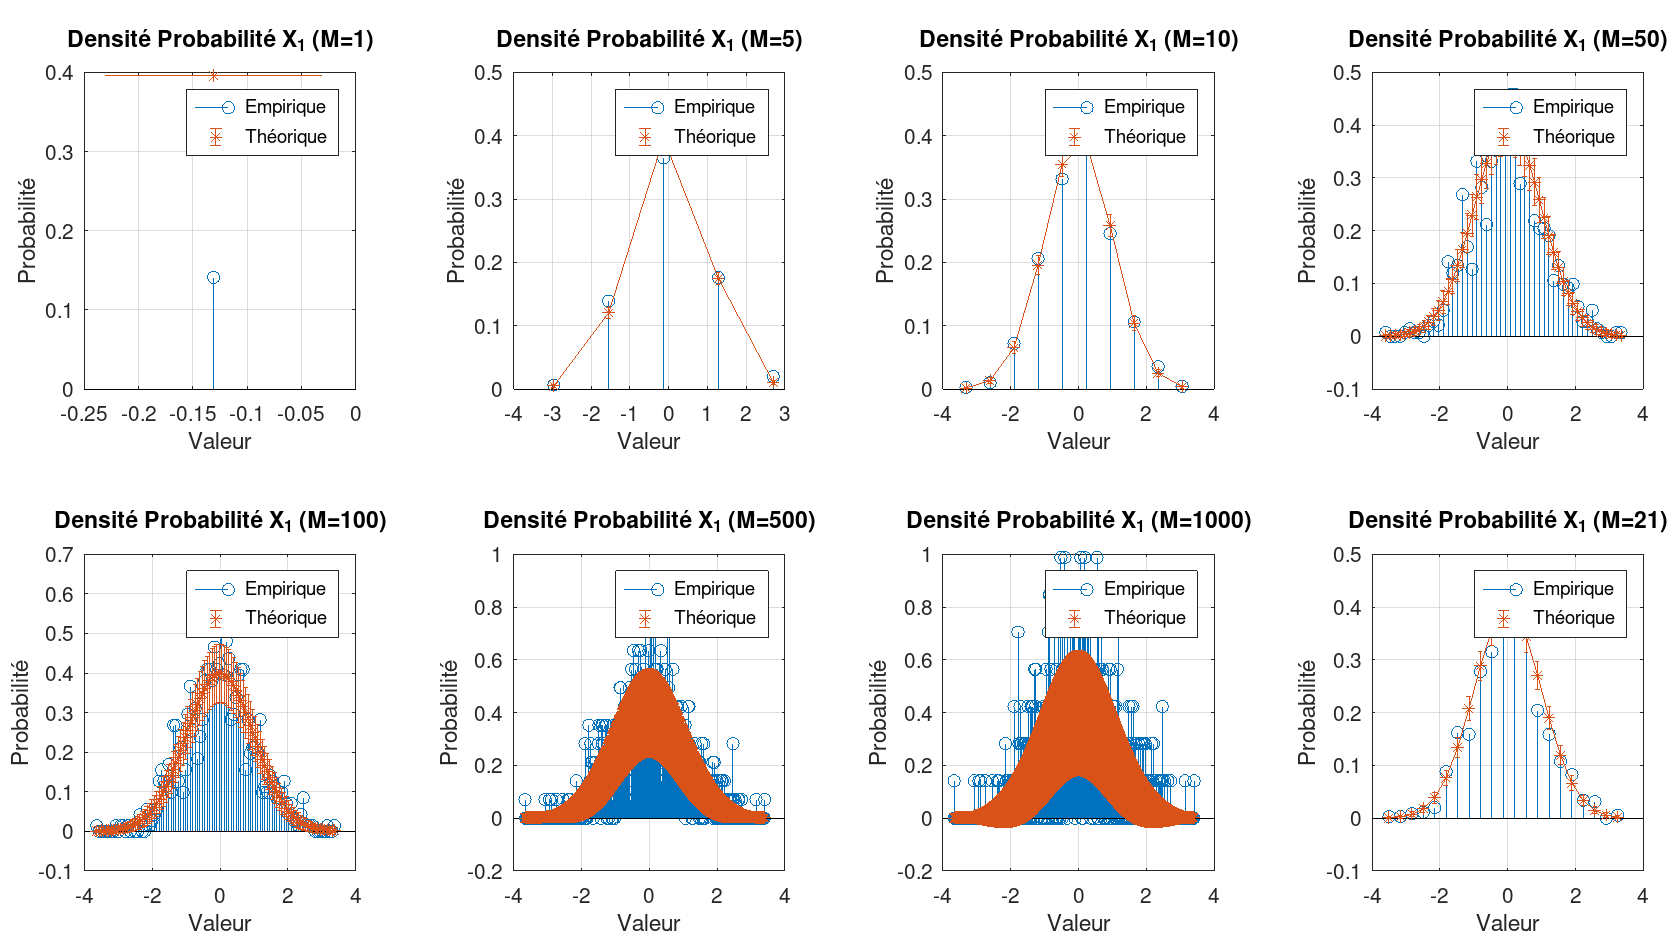
\includegraphics[width=1.15\columnwidth]{Mvar.png}
    \caption{Variation du nombre de classe M}
\end{figure}
\finrep


\item[c)] Comme pour la question précédente, décrivez qualitativement  en l'expliquant, l'évolution de la variance et du biais d'estimation en fonction de $\Delta x$. 

\debutrep{réponse ci-dessous}
On observe comme prévu une augmentation de la variance de l'estimation (quantifiée par les barres rouges) lorsque M augmente (donc $\Delta x$ diminue). On observe dans l'autre cas etrême un écrt significatif entre la valeur théorique et la valeur estimée.
\finrep

\end{list}

\subsubsection{Influence de $B$}

On se place dans les conditions suivantes:

\begin{list}{-}{\setlength{\leftmargin}{3mm} \setlength{\labelwidth}{20mm} \setlength{\labelsep}{2mm} \setlength{\itemsep}{1mm} }
\item $N=1000$ échantillons
\item $m_3 \neq 0$ et $\sigma_3>1$ (garder les mêmes valeurs que celles choisies pour la première expérience)
\item choix empirique {\em optimal} des largeurs d'intervalles $\Delta x$
\item Filtre de Butterworth passe-bas, d'ordre $m=8$ et de \textbf{bande $B=5\,Hz$}.
\end{list}

\begin{list}{}{\setlength{\leftmargin}{6mm} \setlength{\labelwidth}{20mm} \setlength{\labelsep}{2mm} \setlength{\itemsep}{1mm} }

\item[a)]  Afficher  sur une même figure dans différents sous-graphes, le gabarit (gain complexe) du filtre passe-bas correspondant, le processus filtré $x_2(t)$  et la densité de probabilité estimé sur le processus filtré $x_2(t)$. \textbf{Superposer la densité théorique}.

\debutrep{figures ci-dessous}
\begin{figure} [H]
    \centering
    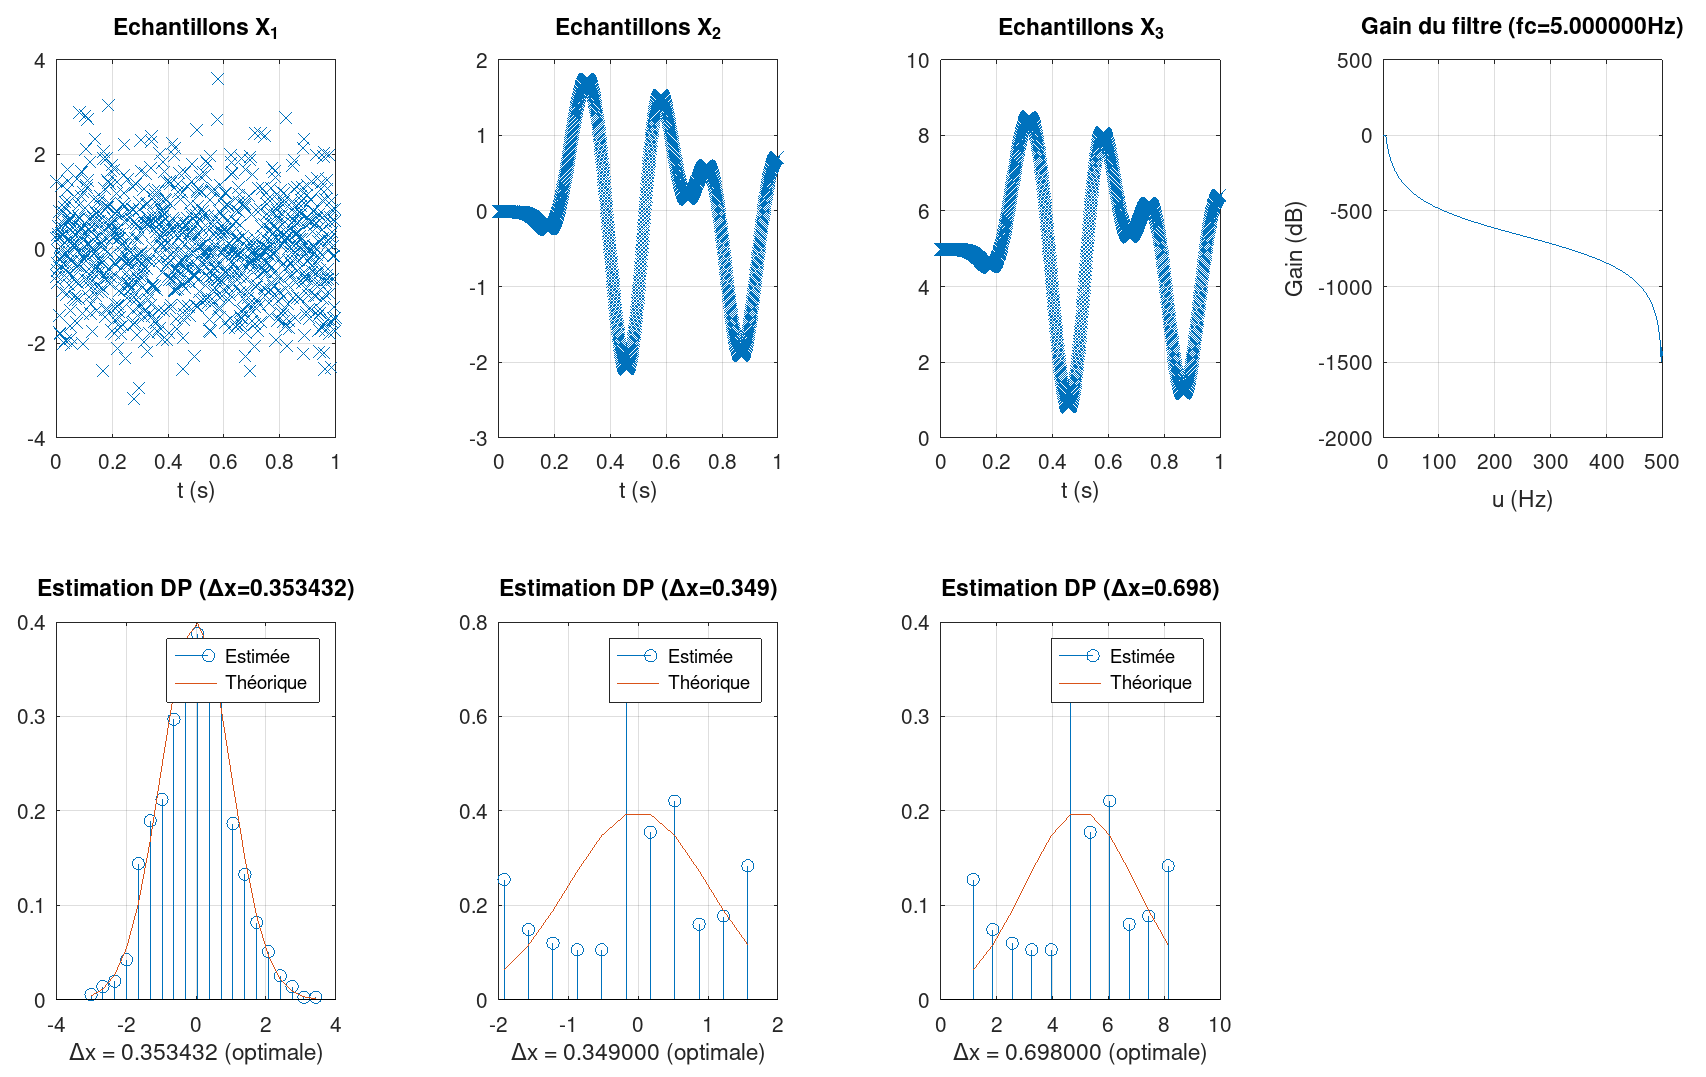
\includegraphics[width=1.15\columnwidth]{Bvar.png}
    \caption{Variation de la fréquence de coupure $f_c$}
\end{figure}
\finrep


\item[b)]  Le signal $x_2(t)$ est il gaussien? Justifiez votre réponse (on pourra par exemple calculer le 
\debutrep{réponse ci-dessous}
Kurtosis sur la série temporelle $\left(x_2[n]\right)_{n=1,\ldots N}$).
Au vu de la forme de la densité de probabilité au regarde de la densité théorique, on peut déduire facilement que le signal n'est pas gaussien.
On peut également le confirmer en calculant le Kurtosis de cette estimation. Un signal gaussien a un Kurtosis valant 3. Le signal considéré lui a un Kurtosis égal à $2.0373$.
\finrep

 
\item[c)] Pourquoi l'estimation de la densité de probabilité de $x_2$ est elle aussi différente de la densité gaussienne $\mathcal{N}(m_2,\sigma_2)$? En gardant  $B=5\,Hz$, proposer une nouvelle configurations de paramètres pour corriger cet effet. Vérifier la solution proposée, \textbf{en affichant la densité de probabilité ainsi estimée}.

\debutrep{réponse ci-dessous}
La différence vient à cause du filtrage. En effet, le filtrage passe-bas réduis la bande spectrale $B$ du signal. Le rayon de corrélation augmente alors en conséquence. Les échantillons sont alors de plus en plus corrélés. Si le nombre d'échantillons est faible, on n'observe plus alors d'échantillons décorrelés et l'hypothèse d'ergodicité n'est alors plus respectée. L'estimation échoue alors.

Pour contrer l'effet du filtrage, on peut alors augmenter le nombre d'échantillons observés de sorte à continuer d'observer des échantillons décorrelés même si le rayon de corrélation augmente.

On simule ci-dessous ce cas avec $N=1e5$ et $B=5Hz$. On retrouve alors la bonne estimation.
\finrep

\debutrep{figures ci-dessous}
\begin{figure} [H]
    \centering
    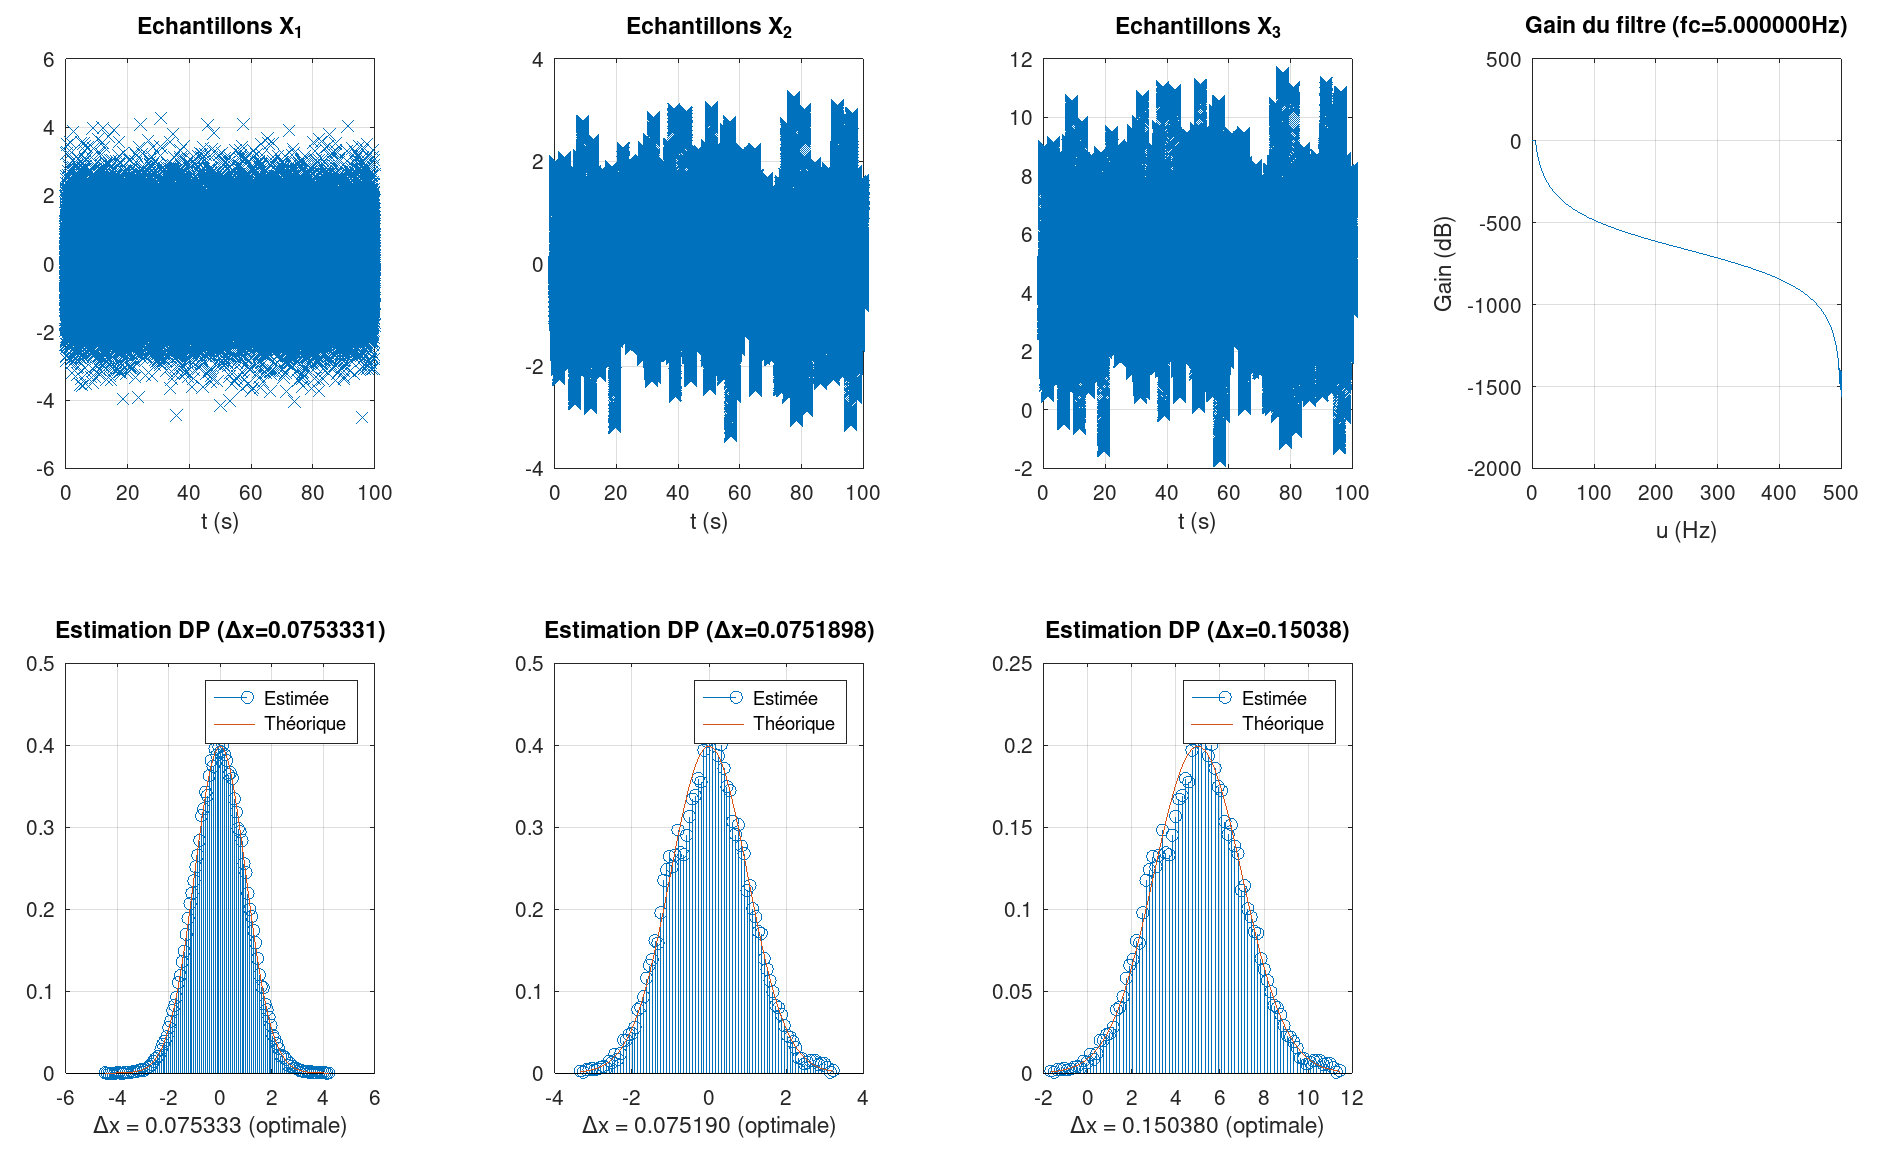
\includegraphics[width=1.15\columnwidth]{NaugBvar.png}
    \caption{Augmentation du nombre d'échantillons N avec filtrage très sélectif}
\end{figure}
\finrep


\end{list}

\clearpage 
\section{\mbox{Somme d'un signal carré à retard équiparti et d'un bruit gaussien}}

On veut étudier la densité de probabilité de la somme d'un signal carré à retard équiparti $\mathbf{y}$ et d'un bruit gaussien  $\mathbf{x}$ de valeur moyenne $m_B$ et d'écart-type $\sigma_B$.\\

Pour cela, utiliser la fonction Matlab {\tt carbr(moy,ecartype,N)}, où:
\begin{list}{}{\setlength{\leftmargin}{20mm} \setlength{\labelwidth}{20mm} \setlength{\labelsep}{3mm} \setlength{\itemsep}{1mm} }
\item[{\tt moy:}] moyenne du bruit
\item[{\tt ecartype:}] écart-type du bruit
\item[{\tt N:}] nombre de points de signal à analyser
\end{list}

Le signal carré, de fréquence $\nu_0=110\,Hz$, d'amplitude $\pm 1$, a pour  retard à l'origine, une variable aléatoire $\tau$ distribuée uniformément sur l'intervalle $[0,T_0[$, où $T_0=1/\nu_0$ est la période du signal carré. \\

En quelques mots, expliquer alors, en quoi le signal carré est un signal aléatoire? \\

\debutrep{réponse ci-dessous}
On nous dit dans l'énoncé que le retard à l'origine de notre signal carré est géré par $\tau$ qui est une variable aléatoire. Celà signifie concrètement que pour plusieurs essais de notre signal carré, on peut ne pas avoir la même valeur pour un instant t donné. Celà est due au fait qu'on ne "démarre" pas le signal au même endroit de notre période.\\Notre signal carré est donc un signal aléatoire.
\finrep


La somme $\mathbf{z}$ des 2 signaux aléatoires est échantillonnée à 100 kHz. \\
La fonction affiche le mélange signal carré $+$ bruit et la d.d.p. estimée $\widehat{P_{\mathbf{z}}}(z)$.\\

En choisissant la moyenne du bruit $m_B=0$, trouver, en la justifiant, la valeur de l'écart-type $\sigma_B$ correspondant à chacune des 2 situations suivantes:
\begin{list}{}{\setlength{\leftmargin}{10mm} \setlength{\labelwidth}{20mm} \setlength{\labelsep}{3mm} \setlength{\itemsep}{1mm} }

\item[1)] $\mathbb{P} \{z \in [-0.5,0.5]\} \leq 0.5 \%$

\debutrep{réponse ci-dessous}
On échantillone a bien plus que $2\nu_0$ donc il n'y aura donc pas de repliement spectral.
Le signal étant de carré d'amplitude $\pm 1$ et de rapport cyclique 0.5, sa moyenne est nulle. Le bruit gaussien ayant une moyenne nulle, notre signal a donc une moyenne de $\sigma=0$.\\
On a donc $\mathbb{P} \{z \in [-0.5,0.5]\} = 2\mathbb{P} \{z \in [0,0.5]\}$

\begin{itemize}
    \item Si $y=1$:
        \[
        \begin{split}
            \text{On a }\mathbb{P} \{z \in [0,0.5]\}=\mathbb{P} \{x<-0.5\}
        \end{split}
        \]
    \item si $y=-1$:
        \[
        \begin{split}
            \text{On a } \mathbb{P} \{z \in [0,0.5]\}=\mathbb{P} \{x>0.5\}
        \end{split}
        \]
\end{itemize}
Comme x est un bruit blanc et que le rapport.

$\mathbb{P} \{x<-0.5\} = \mathbb{P} \{x>0.5\}$

Le rapport cyclique est de 0,5 ces deux cas sont similaires en terme de probabilités, en sommant on obtient finalement

$\mathbb{P} \{z \in [-0.5,0.5]\}=\mathbb{P} \{x<-0.5\}$

On pose T la variable réduite:

$\mathbb{P} \{T<\frac{-0.5}{\sigma_B}\}=0,5$

Et d'après le tableau
$\sigma_B = 1/(2*3) = 1/6$




\newpage
En utilisant le tableau de la loi normale ci dessous

\begin{figure} [H]
    \centering
    \includegraphics[width=\columnwidth]{Loi Normale.png}
    \caption{Densité de probabilité d'une loi normale}
\end{figure}


\finrep

\item[2)] ${\displaystyle p_{\mathbf{z}}(0) = \frac{1}{2} \, p_{\mathbf{x}}(0)}$

\debutrep{réponse ci-dessous}
On raisonne avec la largeur a mis hauteur.
\[
p_{\mathbf{z}}(0) = \frac{1}{2}(  p_{\mathbf{x}}(1)+ p_\mathbf{x}(-1))=p_{\mathbf{x}}(1)\\
\]

On peut maintenant utiliser les propriétés de la mi hauteur de la gaussienne sachant que:
\[
{\displaystyle p_{\mathbf{x}}(0) = \frac{1}{2} \, p_{\mathbf{x}}(0)}
\]

On a donc $\sigma_b= \frac{2}{2.35}=0.85$ 

\finrep

\end{list}

\textbf{Afficher sur une même figure, les deux densités correspondantes.}

\debutrep{figures ci-dessous}

\begin{figure} [H]
    \centering
    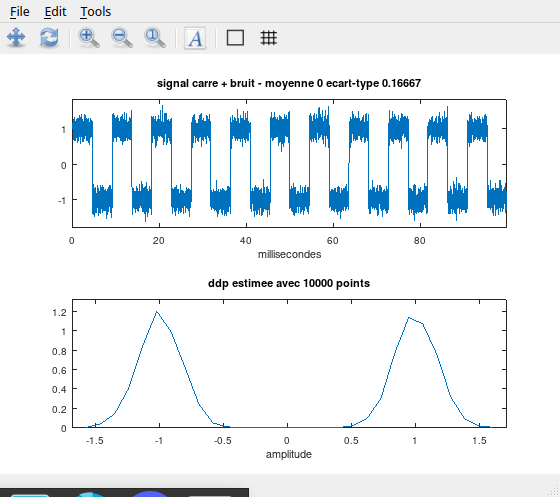
\includegraphics[width=\columnwidth]{Part3-1.png}
    \caption{Densité de probabilité d'une loi normale}
\end{figure}

\begin{figure} [H]
    \centering
    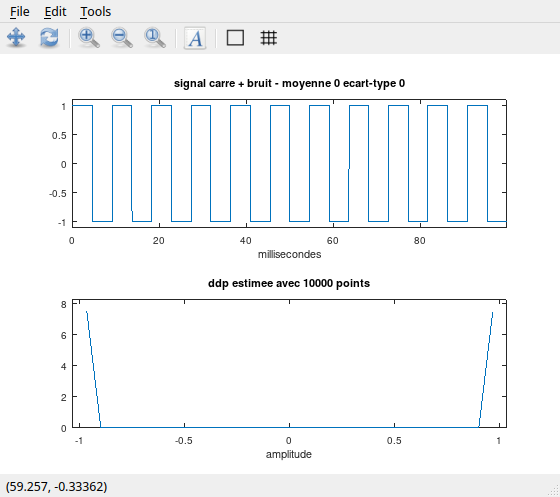
\includegraphics[width=\columnwidth]{Part3-2.png}
    \caption{Densité de probabilité d'une loi normale}
\end{figure}

\finrep

\end{document}








































